%% marcel's template

\documentclass[12pt]{article}
\usepackage[margin=0.5in]{geometry}
\usepackage{amsmath,amsthm,amssymb,amsfonts,tikz,tikzsymbols}
\usepackage[shortlabels]{enumitem}

\usepackage{hyperref}

\newenvironment{rcases}
  {\left.\begin{aligned}}
  {\end{aligned}\right\rbrace}

\newcommand{\N}{\mathbb{N}}
\newcommand{\Z}{\mathbb{Z}}
\newcommand{\Q}{\mathbb{Q}}
\newcommand{\R}{\mathbb{R}}
\newcommand{\C}{\mathbb{C}}
\newcommand{\F}{\mathbb{F}}
\newcommand{\RA}{\Rightarrow}

\newcommand{\M}{\mathbb{M}}

\renewcommand\qedsymbol{$\Smiley$}

\newenvironment{problem}[2][Question]{\begin{trivlist}
\item[\hskip \labelsep {\bfseries #1}\hskip \labelsep {\bfseries #2.}]}{\end{trivlist}}
\newenvironment{exercise}[2][Exercise]{\begin{trivlist}
\item[\hskip \labelsep {\bfseries #1}\hskip \labelsep {\bfseries #2.}]}{\end{trivlist}}
%If you want to title your bold things something different just make another thing exactly like this but replace "problem" with the name of the thing you want, like theorem or lemma or whatever

\begin{document}
 
%\renewcommand{\qedsymbol}{\filledbox}
%Good resources for looking up how to do stuff:
%Binary operators: http://www.access2science.com/latex/Binary.html
%General help: http://en.wikibooks.org/wiki/LaTeX/Mathematics
%Or just google stuff
 
\title{DATA SILSO HISTO quality control Report}
\author{Stephen Fay}
\maketitle

\section{Introduction}
\subsection{Github repository and project}
    https://github.com/dcxSt/DATA\_SILSO\_HISTO\_search \\
    https://github.com/users/dcxSt/projects/2?fullscreen=true
    
\subsection{Brief History et Mise en Contexte}

For centuries we have observed the sun and it's ever mysterious sunspots. The 11 year sunspot cycle has long been a subject of debate. Today we wish to have precise quantification of solar activity throughout the previous centuries. This is made possible by the sunspot series. For the past 3 to 4 hundred years people all over the Eurasian continent have been recording the number of sunspots that appear on the sun's earth facing half. 

The aim of this project is to do a quality control of the data in DATA\_SILSO\_HISTO. Once the data is fixed and cleaned up, it will be stored on a new database - temporarily named GOOD\_DATA\_SILSO in a more user-friendly format to what currently exists. I will also get rid of any useless or redundant columns (such as the observers comment column - there are no comments )': ). A third, temporary database will be mad to keep a closer eye on the data that still needs to be examined with more scrutiny : BAD\_DATA\_SILSO. This database will act as intermediary between DATA\_SILSO\_HISTO and GOOD\_DATA\_SILSO. We will effectively be storing 2 databases-worth of information in 3 databases. The original DATA\_SILSO\_HISTO will have the old data and will be corrected in due course. The intermediary BAD\_DATA\_SILSO will start as a copy of DATA\_SILSO\_HISTO and end up empty as the corrected data is removed from it and placed, in the new format, into GOOD\_DATA\_SILSO.


\section{Processus de filtration / corigee du data (log) / quality control}

\subsection{Everything wrong with the data}

First, it's important to note that note that though I am doing a quality control I do not wish to die of boardom. I will not be verifying each of the 205003 data-points by hand in the Mittheilungen journals, in any case this if I went about it this way I would probably miss most of the errors.

\subsection{Annotation keys}

\subsubsection{What do the flags mean?}\label{flags section}
\newpage% idk how to make tables behave!
\begin{table}[h!]
    \centering
    \begin{tabular}{c|c|c|c|c|c|c|c|c|c}
        0 & 1 & 2 & 3 & 4 \\
        same as Null & suspicious & Comment in journal = ? & move to bin & slightly suspicious\\
        \hline
        5 & 6 & 7 & 8 & 9\\
        definitely erroneous & na & probs ok, to be investigated & na & na
         
    \end{tabular}
    \caption{Flags key}
    \label{tab:flag}
\end{table}
\begin{enumerate}[start=0]
    \item The default for the flag is NULL, when is estimate that the datapoint is perfect and there is nothing wrong with it, I can put it to zero 0.
    \item If the data looks fishy but I'm not quite sure either what is wrong with it or how wrong it is this is flagged with a 1 - the default.
    \item If in the Mitteilungen journals there is written a ? next to one of the data points, I will mark it with a 2, this means that the observer is not quite confident in his/her result.
    \item A flag that signifies that this data point is definitely going into the bin
    \item For data that is very dodgy but it is ambiguous as to weather or not it is correct, to determine its validity closer examination is required
    \item For data that is definitely wrong, the difference between 5 and 4 is illustrated by example: if i find that a datapoint has a groups number of 30 I will mark it with a 4 and comment it, because this is suspicious, if a datapoint has a groups number over 60 or above, it will be marked with a 5 (trust me there are some in the hundreds).
\end{enumerate}
  


\subsection{Search and correct.}

\subsubsection{Outline}

For the first week and a half or so, I spent the bulk of the time acquainting myself with the Mittheilungen journals, and with the software that is used to store and access the database. I also developed the tools in python to facilitate my access to them and to perform the tasks that I need to perform for the filtration process. 



\subsubsection{Log}
I started this (today) on 2019.06.21 (yes, the solstice!)
\begin{itemize}
    \item Friday June 21
    \begin{itemize}
        \item Today no-one was in the office in the morning so I didn't have access to the Mittheilungen journals and decided to start writing this instead
        \item at 10:20 I was let into my bit with all my notes and the journals and began 'searching the manuals' part of the project documented in the Github project linked
        \item been spending time writing in all the pink corrections, including typos
        \item started writing 'searching\_the\_manuals.py'
        \item wrote and executed methods : def\_correct\_typos\_for\_pink() ; pink()
        \item searching the manuals for all comments labeled 'uncertain' so as to figure out what is this word's range of meaning (wishing I had paid attention in German class)
    \end{itemize}
    \item Monday June 24
    \begin{itemize}
        \item 9.15 picking up from where I left off, I am currently scouring the manuals for any 'uncertain' data
        \item 10.40 came across some duplicate data, and mysterious comments... there are some stars '*' that signify a change of instrument but nothing is written. The annoying thing about the duplicate data is that it is coming from 
        \item spent the morning making that duplicate finding and sorting algorithm, now I need to analyse the nature of the problem further. For each of the duplicates identify what kind it is, weather it's the same observer with the same instrument; if the duplicated data has for example the same rubrics numbers as each other ; if they record the same information (sunspot groups, sunspots, wolf number) ; if check to see if any clues are hidden in the comments of these duplicated data
        \item in searching\_the\_manuals i wrote : find\_duplicate\_observers() ; find\_obs\_id\_by\_date() ; find\_observer\_alias\_by\_id() ; find\_duplicates\_data() ; write\_greater\_duplicates\_data\_text()
        \item i'm gonna go and delete some of the data so i will log everything in order to be very careful
    \end{itemize}
    \item Tuesday June 25
    \begin{itemize}
        \item 9.45 I have decided to start making modifications to the database, this is risky business - I don't want to have the blood of Galileo's data on my hands, in a few seconds I can destroy hours upon hours of one of my predecessors' work. Which would be a shame. This is why I am creating a new table in both the old and the new database that will serve as a rubbish bin, so that I simultaneously copy and delete some data. The data will be copied and destroyed in the same script but the coping will come \textit{before} so if there are bugs nothing will be lost. First I will back up the databases as they are.
        \item While making the rubbish bids for DATA\_SILSO\_HISTO if found that DATA\_DEV was non-empty, it contains data which claims to be observations made by the grandfather of this series - Rudolf Wolf. Only the observations are dated January 1600 - Galileo's time, 216 years before Wolf's birth! And so I renamed the DATA\_DEV to RUBBISH\_DATA and added the flag column, leaving those four observations inside where they probably belong...
        \item Wrote a new script to deal uniquely with deleting the duplicates
        \begin{itemize}
            \item finished writing move\_data\_to\_bin and delete\_entered\_twice\_duplicates
            \item executing delete\_entered\_twice\_duplicates()... done
            \item finished commenting these data points in rubbish data in both databases
        \end{itemize}
    \end{itemize}
    \item Wednesday June 26
    \begin{itemize}
        \item wrote a new method in db\_edit for appending comments rather than replacing them
        \item wrote \textit{unreasonable\_sn\_flag()} a method that takes a look at the groups number and the sunspots number of each entry and determines if it's realistic or not. I decided somewhat arbitrarily that if the groups number was higher than 30 it would be flagged with flag 4, if the groups number was higher than 60 it would be marked with a 5 this is beyond unreasonable. I did something similar for the sunspots number $sunspots>100\Rightarrow flag:=4$ and $sunspots>250\Rightarrow flag:=5$ (see the flags section \ref{flags section}). The method was executed and ran without a hitch (after a bit of debugging)
        \item just set another 212 flags for putting things in the bin. There are still 4000 pairs of duplicates that need attending to but considering i started with 14000 that's not bad... Some of the duplicates may be left as they are. Also i figured out that i had flagged some which just had a 0 sunspot number and so i went and unflagged them.
        \item i spent alot of time scrutinising what i had flagged, rereading my scripts, seeing that I've been using really inefficient algorithms, checking things are in the right place. And wondering how on earth many things ended up with the flags they ended up with.
        \item something that has been annoying me in this search is I can't seem to be able to determine what is an unreasonable number of sunspots that can appear on the sun, because many many observer record having over 250. This is why I will start using graphical tools to help me figure all of this out. I will make the graphs in a jupyter notebook.
    \end{itemize}
    \item Thursday June 27
    \begin{itemize}
        \item first thing i did today is to go though and look at lots of the flagged data from yesterday on the mysql databases
        \item Panic! While searching I came across a big problem. Many of the datapoints are labelled '*' in the comments, this corresponds to when there is an asterix in the Mitteilungen journals, but here's the twist: the star is usually a reference to the fact that there is a change in the observer's telescope to his/her secondary lunette. This is written nowhere is many cases in the digital database! This is a new task I must take on am I to accomplish my mission here:
        \begin{enumerate}
            \item Correct all the comments so that they display useful information i.e. '*' --- '* = 8 cm Oeffnung mit 64-facher Vergrosserung und Polarisationshelioscop'
            \item When you tackle the 'Creating New Aliases' part of the project (see my Github - username = dcxSt - project sun)
        \end{enumerate}
        \item I found there I had flagged all the mysterious '*' comment 1 and that none of them have found their way into my pristine database GOOD\_DATA\_SILSO and so I went through each of them individually and wrote the changes that I implemented in the python method 'correct\_asterix\_comments()' in script 'db\_homogenise\_comments.py'. This took quite some time and included translating German with my good friend google-translate. This corrected about 250 data-points' comments (i didn't bother to count)
        \item after a long search of the data in GOOD\_DATA\_SILSO with FLAG=3 which have no superior duplicates I found that these were infact correctly flag and that their double had not yet made it into my new database because there were commented (usually with an asterisk *) so i moved them into the bin
        \item Found a bug in move\_flag3\_to\_bin() which may have been causing some of the perplexing problems I had earlier
        \item I ran the method 'flag\_many\_duplicates()' many times using the duplicates text files I'd made earlier for inspiration to change it subtly so as to catch those sneaky no good duplicates!
        \item IMPORTANT: I just found some data which has been written in in the wrong year. In rubrics 820 students have mistakenly typed in the data for Wolfer in the year 1900 and written it in the year 1899.
        \item In the folder duplicates/3 2019.06.27 I am writing the file corrections\_needed\_handwritten.txt which outlines the corrections which are to be made to the data if we want to solve some of these duplicates.
    \end{itemize}
    
\end{itemize}

\subsubsection{Python scripts - what they contain}



\section{Comparaison du data avant et apres + visualisations}

\subsubsection{The original sql data tables format}

\begin{table}[h!]
    \centering
    \caption{DESCRIBE DATA}
    \begin{tabular}{c|c|c|c|c|c}% l c r = Left Centre Right
        \textbf{Field} & \textbf{Type} & \textbf{Null} & \textbf{Key} & \textbf{Default} & \textbf{Extra}  \\
        \hline
        ID & int(11) & No & PRI & NULL & auto\_increment \\
        
        DATE & date & YES && NULL & \\
        
        FK\_RUBRICS & int(11) & YES & MUL & NULL &  \\
        
        FK\_OBSERVERS & int(11) & YES & MUL & NULL &  \\
        
        GROUPS & int(11) & YES && NULL &  \\
        
        SUNSPOTS & int(11) & YES && NULL & \\
        
        WOLF & int(11) & YES && NULL &  \\
        
        QUALITY & int(11) & YES && NULL &  \\
        
        COMMENT & text & YES && NULL &  \\
        
        DATE\_INSERT & datetime & YES && NULL &  \\
        
        FLAG (i added this) & tinyint(1) & YES && NULL &  \\
        
    \end{tabular}
    \label{tab:data-og}
\end{table}

\begin{table}[h!]
    \centering
    \caption{DESCRIBE OBSERVERS}
    \begin{tabular}{c|c|c|c|c|c}% l c r = Left Centre Right
        \textbf{Field} & \textbf{Type} & \textbf{Null} & \textbf{Key} & \textbf{Default} & \textbf{Extra}  \\
        \hline
        ID & int(11) & NO & PRI & NULL & auto\_increment \\
        
        ALIAS & varchar(50) & YES && NULL & \\
        
        FIRST\_NAME & varchar(50) & YES && NULL &  \\
        
        LAST\_NAME & varchar(50) & YES && NULL &  \\
        
        COUNTRY & varchar(50) & YES && NULL &  \\
        
        INSTRUMENT & varchar(50) & YES && NULL & \\
        
        COMMENT & text & YES && NULL &  \\
        
        DATE\_INSERT & datetime & YES && NULL &  \\
        
    \end{tabular}
    \label{tab:data-og}
\end{table}

\begin{table}[h!]
    \centering
    \caption{DESCRIBE RUBRICS}
    \begin{tabular}{c|c|c|c|c|c}% l c r = Left Centre Right
        \textbf{Field} & \textbf{Type} & \textbf{Null} & \textbf{Key} & \textbf{Default} & \textbf{Extra}  \\
        \hline
        RUBRICS\_ID & int(11) & NO & PRI & NULL & auto\_increment \\
        
        RUBRICS\_NUMBER & int(11) unsigned & NO && NULL & \\
        
        MITT\_NUMBER & int(11) unsigned & NO && 0 &  \\
        
        PAGE\_NUMBER & int(11) unsigned & YES && NULL &  \\
        
        SOURCE & text & NO && NULL &  \\
        
        SOURCE\_DATE & date & YES && NULL & \\
        
        COMMENTS & text & YES && NULL &  \\
        
        DATE\_INSERT & datetime & YES && NULL &  \\
        
        NB\_OBS & int(11) & YES && NULL & \\
        
    \end{tabular}
    \label{tab:data-og}
\end{table}

\newpage{}

\subsubsection{My new sql data table format}

\begin{table}[h!]
    \centering
    \caption{DESCRIBE DATA (the only table)}
    \begin{tabular}{c|c|c|c|c|c}% l c r = Left Centre Right
        \textbf{Field} & \textbf{Type} & \textbf{Null} & \textbf{Key} & \textbf{Default} & \textbf{Extra}  \\
        \hline
        ID & int(11) unsigned & No & PRI & NULL & auto\_increment \\
        
        DATE & date & YES && NULL & \\
        
        GROUPS & int(11) & YES && NULL &  \\
        
        SUNSPOTS & int(11) & YES && NULL & \\
        
        WOLF & int(11) & YES && NULL &  \\
        
        COMMENT & text & YES && NULL &  \\
        
        DATE\_INSERT & datetime & YES && NULL &  \\
        
        OBS\_ALIAS & varchar(50) & YES && NULL & \\
        
        FIRST\_NAME & varchar(50) & YES && NULL & \\
        
        LAST\_NAME & varchar(50) & YES && NULL & \\
        
        COUNTRY & varchar(50) & YES && NULL & \\
        
        INSTRUMENT\_NAME & varchar(50) & YES && NULL & \\
        
        RUBRICS\_NUMBER & int(11) & YES && NULL & \\
        
        MITT\_NUMBER & int(11) & YES && NULL & \\
        
        PAGE\_NUMBER & int(11) & YES && NULL & \\
        
        FLAG & tinyint(1) unsigned & YES && NULL &  \\
        
        RUBRICS\_SOURCE & text & YES && NULL & \\
        
        RUBRICS\_SOURCE\_DATE & date & YES && NULL & \\
        
    \end{tabular}
    \label{tab:data-og}
\end{table}





\newpage{}

\subsubsection{Graphs and visual representations}

As you can see, there are some famous legends in solar science such as Carrington and Kew who were able to see over 4000 sunspots at once on a single face of the sun with their crappy telescopes that they had in the 19th century!
\begin{figure}
  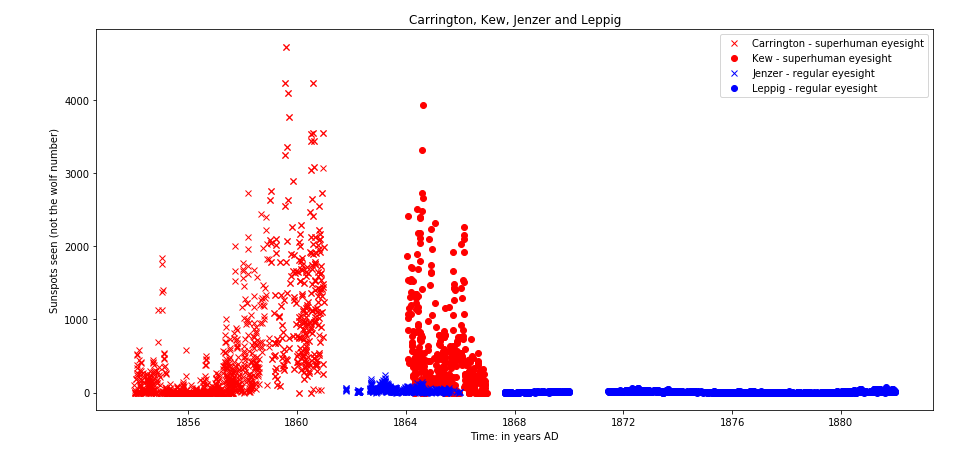
\includegraphics[width=\linewidth]{CarringtonHasGoodEyesight.png}
  \caption{Carrington has great eyesight!}
  \label{fig:boat1}
\end{figure}

\subsubsection{Thought repository - ideas that may or may not come into fluition depending on how efficiently I work and get things that need to be done done}
\begin{itemize}
    \item make some data visualisations to compare each observer's primary and secondary observing equipment
    \item for each day / month / year find the highest observation and the lowest observations and add it to the graph so that we have like an upper bound and a lower bound. 
    \item figure out how to smooth graphs with matplotlib and make something nice out off the big mess i currently have
    \item pie chart of observers with their number of observations
    \item in the final sunspots number graph cut it into 3 or 4 sections that mark changes in the theory behind sunspots: before wolf ; time where plato's ideas of the sun being a perfect sphere still were around ; 1908 George Ellery Hale discovers the magnetic link (p14 of nature's 3rd cycle) ; 1955 eugene parker's theory (p19 of nature's 3rd cycle) ; Nasa send their probe to near the sun
\end{itemize}

\end{document}